\documentclass[11pt,a4paper]{article}
\usepackage[margin=2.3cm]{geometry}
\usepackage[T1]{fontenc}
\usepackage{textcomp}
\input{glyphtounicode}
\pdfgentounicode=1
\usepackage{lmodern}
\usepackage{xcolor}
\usepackage{listings}
\usepackage{tcolorbox}
\usepackage{booktabs}
\usepackage{array}
\usepackage{graphicx}
\graphicspath{{images/}}
\usepackage{hyperref}
\hypersetup{colorlinks=true, linkcolor=blue!50!black, citecolor=green!40!black}

\definecolor{codebg}{RGB}{248,248,245}
\lstset{
  language=C, basicstyle=\ttfamily\footnotesize, backgroundcolor=\color{codebg},
  keywordstyle=\color{blue!60!black}\bfseries, commentstyle=\color{green!45!black}\itshape,
  stringstyle=\color{red!60!black}, numbers=none, upquote=true,
  frame=single, rulecolor=\color{gray!40}, breaklines=true, columns=fullflexible,
  keepspaces=true, showstringspaces=false
}
\lstdefinestyle{sh}{language=bash, backgroundcolor=\color{black!5}}

\newtcolorbox{keyidea}{colback=blue!4, colframe=blue!45!black, title=Key ideas, fonttitle=\bfseries\small}
\newtcolorbox{experiment}{colback=orange!5, colframe=orange!70!black, title=Experiment, fonttitle=\bfseries\small}

\title{\textbf{OpenMP --- Lesson 10}\\[4pt]\large Finding data races with ThreadSanitizer}
\author{Gustavo Lozano}
\date{November 2026}

\begin{document}
\maketitle

\noindent\textit{\small Source: Chapman, Jost \& van der Pas~\cite{chapman}, Ch.~7
``Troubleshooting'' (data races and tools to detect them). Tool documentation: the
ThreadSanitizer and Archer pages of the LLVM project.}

\section{The idea}
Lesson~2 showed that a data race gives wrong results \emph{sometimes}: with small
\texttt{N} the program usually looked correct. Testing the output is therefore not enough
to know that a parallel program is correct. We need a tool that watches the memory
accesses themselves.

\textbf{ThreadSanitizer} (TSan) is built into GCC and Clang. With
\texttt{-fsanitize=thread} the compiler adds a check to every memory access. While the
program runs, TSan records which thread touched which address and which synchronization
(barriers, locks, \ldots) happened in between. When two threads access the same address,
at least one writes, and no synchronization orders them, TSan prints a report with the
file and line of both accesses.

\section{The catch: the tool must understand OpenMP}
TSan knows the synchronization of \texttt{pthreads} (mutexes, thread creation), but
OpenMP runtimes implement barriers and reductions with their own internal tricks. If TSan
cannot see them, it reports races that do not exist (\emph{false positives}).
\begin{itemize}
  \item \textbf{GCC} (\texttt{libgomp}): TSan does not see OpenMP's synchronization, so it
        reports false races even in correct programs.
  \item \textbf{Clang} (\texttt{libomp}) has \textbf{Archer}, a small library that tells
        TSan what OpenMP synchronizes. Load it with the environment variable
        \texttt{OMP\_TOOL\_LIBRARIES}.
\end{itemize}
So for this lesson we use \textbf{Clang + Archer}. On Arch Linux:
\begin{lstlisting}[style=sh]
sudo pacman -S clang openmp compiler-rt
find /usr/lib -name libarcher.so        # check that Archer is installed
\end{lstlisting}

\section{The code}
The buggy counter from Lesson~2, with a smaller \texttt{N} because TSan makes the program
5--15 times slower.
\lstinputlisting[title=\texttt{tsan\_counter.c}]{tsan_counter.c}

\begin{lstlisting}[style=sh]
clang -g -fopenmp -fsanitize=thread -o tsan_counter tsan_counter.c
export TSAN_OPTIONS='ignore_noninstrumented_modules=1'
export OMP_TOOL_LIBRARIES=$(find /usr/lib -name libarcher.so | head -1)
OMP_NUM_THREADS=2 ./tsan_counter
\end{lstlisting}
Output of a real run on Arch Linux (Clang/LLVM 23, \texttt{/usr/lib/libarcher.so}):

\begin{center}
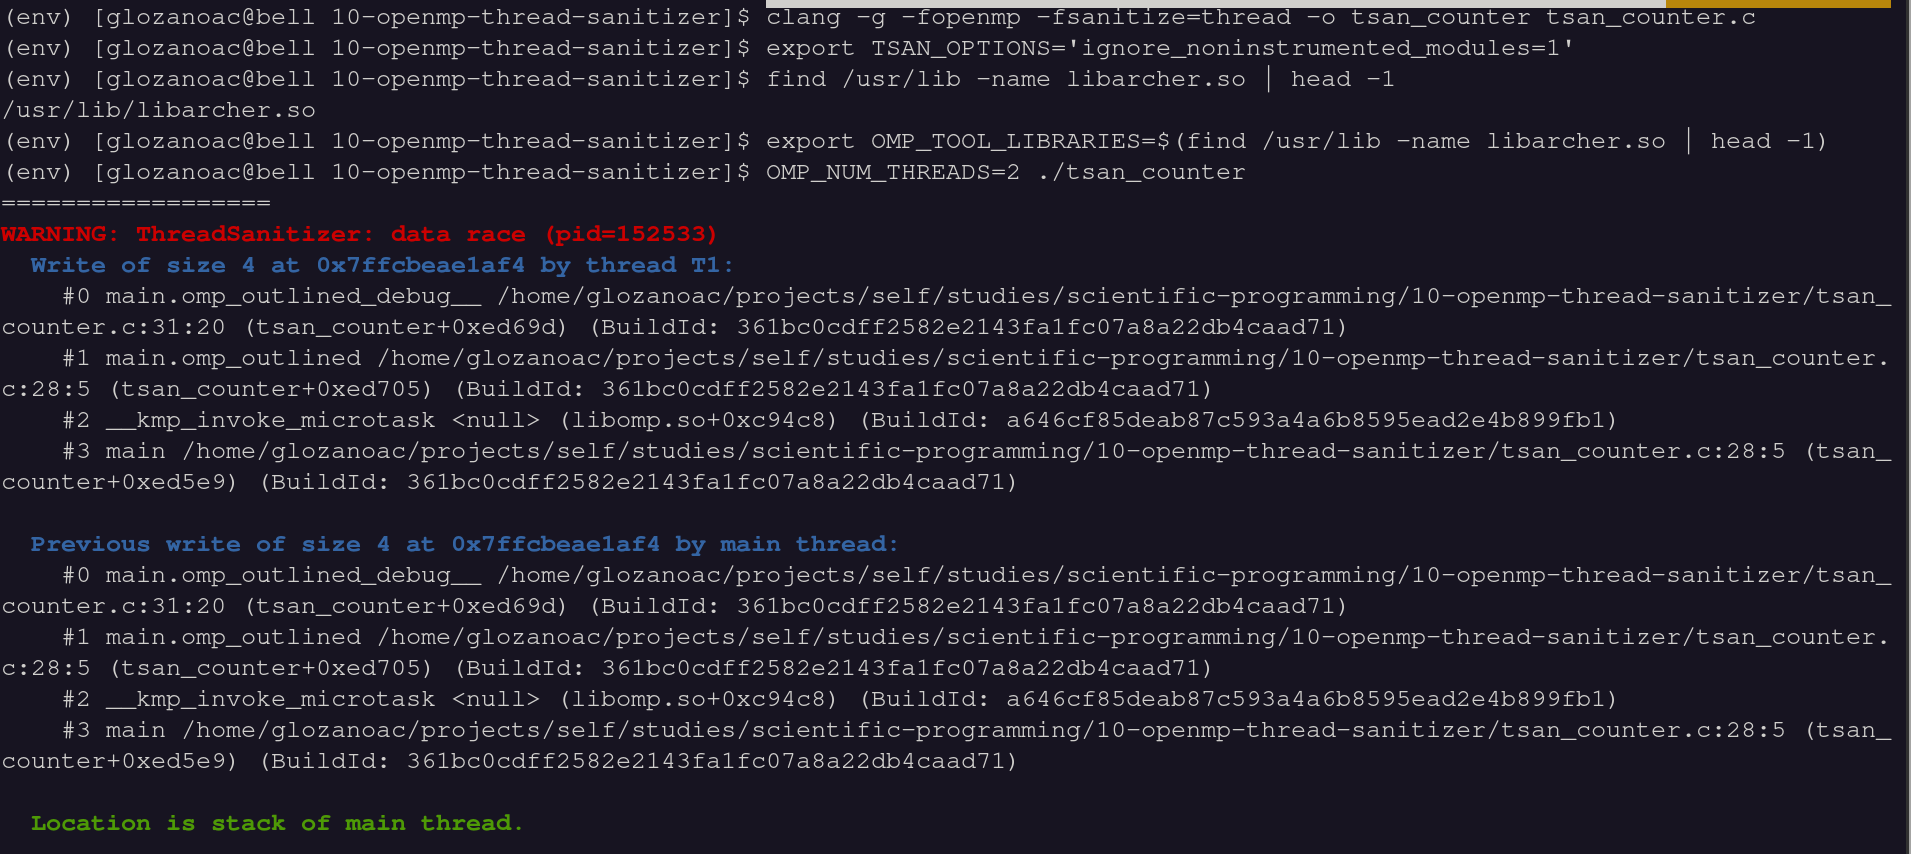
\includegraphics[width=\linewidth]{tsan_report_1.png}\\[2pt]
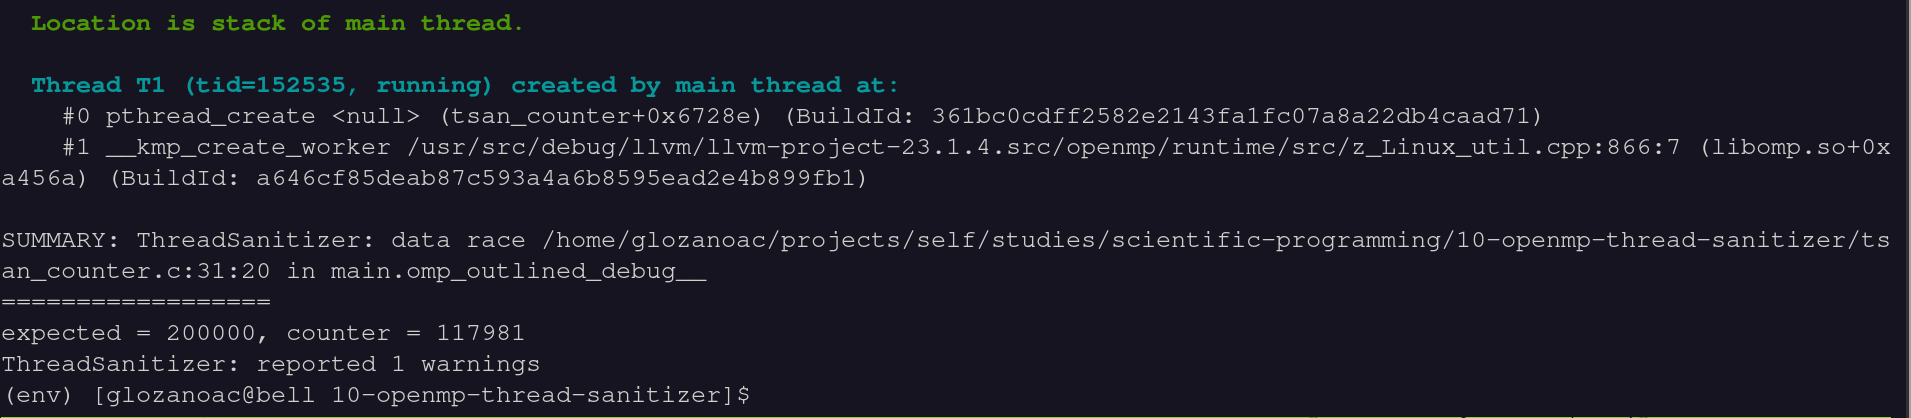
\includegraphics[width=\linewidth]{tsan_report_2.png}
\end{center}

\noindent Note the last lines: in this run the counter is wrong
(\texttt{117981} instead of \texttt{200000}), and TSan reported 1 warning.

\section{Reading the report}
\begin{center}
\small
\begin{tabular}{@{}>{\raggedright\arraybackslash}p{5.0cm}>{\raggedright\arraybackslash}p{10.2cm}@{}}
\toprule
Report line & Meaning \\ \midrule
\texttt{Write of size 4 \ldots by thread T1} & thread T1 wrote 4 bytes (an \texttt{int}) \\
\texttt{\#0 \ldots tsan\_counter.c:31:20} & where: line 31, column 20, the \texttt{counter++} \\
\texttt{Previous write \ldots by main thread} & the conflicting earlier access, by another thread,
  with no synchronization in between \\
\texttt{Location is stack of main thread} & the variable is a local of \texttt{main}:
  \texttt{counter}, shared by default \\
\texttt{\#1 main.omp\_outlined} & \texttt{omp\_outlined} is the function the compiler made from the
  parallel region (\emph{outlining}, Chapman Ch.~8) \\
\bottomrule
\end{tabular}
\end{center}

\begin{keyidea}
\begin{itemize}
  \item TSan points to the exact line and says which threads collided. You no longer guess
        from wrong numbers.
  \item TSan reports the race even in runs where the counter happens to come out
        correct (200000). It detects that a race \emph{can} corrupt the result, not only
        that it did.
  \item Always compile with \texttt{-g}, otherwise the report has no file and line numbers.
  \item Use TSan only for testing: it slows the program down and uses much more memory.
\end{itemize}
\end{keyidea}

\section{The experiment}
\begin{experiment}
\textbf{Question:} can the tool tell a racy program from a correct one?
\begin{enumerate}
  \item Compile and run \texttt{tsan\_counter.c} as above (Clang + Archer). Read the report.
  \item Fix the race: change the pragma to
        \texttt{\#pragma omp parallel reduction(+:counter)}. Recompile with Clang and run
        again, with the same environment variables.
  \item Compile the \emph{fixed} program with GCC instead, and run it:
\begin{lstlisting}[style=sh]
gcc -g -fopenmp -fsanitize=thread -o tsan_gcc tsan_counter.c
OMP_NUM_THREADS=2 ./tsan_gcc
\end{lstlisting}
\end{enumerate}
\textbf{What to observe and answer.}
\begin{enumerate}
  \item In step 1, which line does the report point to? Was the printed counter wrong?
  \item In step 2 there is no report. Does that \emph{prove} the program has no race?
  \item In step 3, GCC's TSan reports a race in the fixed program. Is it real? Why does it
        appear?
\end{enumerate}
\end{experiment}

\noindent Step 2 on Arch Linux (the fixed program saved as \texttt{tsan\_counter\_fix.c}):
the counter is correct and TSan prints no warning.
\begin{center}
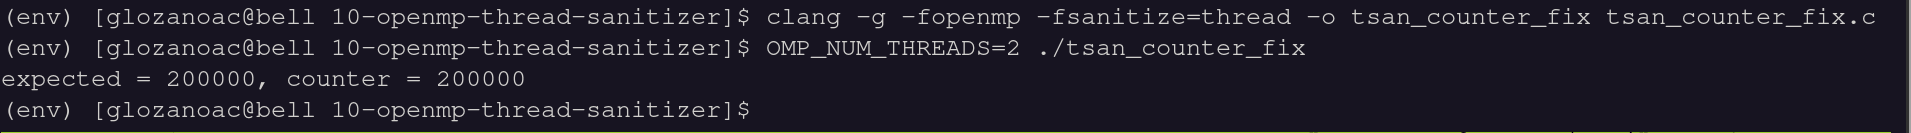
\includegraphics[width=\linewidth]{fix_thread_sanitizer_compiler.png}
\end{center}


\paragraph{Answers (read after trying).}
(1)~Line 31, \texttt{counter++}, written by two threads. The counter may well be correct:
TSan makes the program slow, so the threads interleave less, which hides the wrong result
but not the race. The tool reports the unsynchronized accesses, whatever the result.
(2)~No. TSan is a \emph{dynamic} tool: it only checks the accesses that actually happen in
this run, with this input and these threads. A race in code that this run never executed
is not reported. Silence means ``no race seen'', which is strong evidence but not proof.
(3)~It is a false positive. \texttt{libgomp} combines the private copies of the reduction
with its own internal synchronization, which TSan does not see, so it looks like an
unprotected write. Lesson: a race detector must understand the threading library. For
OpenMP, use Clang with Archer, or a dedicated tool such as Intel Inspector.

\paragraph{Next lesson.} This closes the Chapman book. Next we move to van der Pas et
al.~\cite{vdp}: tasks (\texttt{task} and \texttt{taskwait}), for parallel work that is not
a loop.

\begin{thebibliography}{9}
\bibitem{chapman} B.~Chapman, G.~Jost, and R.~van der Pas. \emph{Using OpenMP: Portable
  Shared Memory Parallel Programming}. MIT Press, Cambridge, MA, 2007.
\bibitem{vdp} R.~van der Pas, E.~Stotzer, and C.~Terboven. \emph{Using OpenMP --- The Next
  Step: Affinity, Accelerators, Tasking, and SIMD}. MIT Press, Cambridge, MA, 2017.
\end{thebibliography}
\end{document}
